\chapter{lImporter}\label{chapter:proposal}
Este capítulo presenta la propuesta de \textit{lImporter}, un plugin para Obsidian diseñado para automatizar la integración de nuevo conocimiento en una bóveda existente. El sistema recibe un conjunto de archivos y, guiado por instrucciones del usuario, genera y vincula nuevas notas de manera inteligente.

El problema fundamental que se aborda puede definirse formalmente. Se construye un Agente, $A$, que opera sobre una bóveda de Obsidian. La función del agente es transformar la bóveda a un nuevo estado basándose en un conjunto de archivos de entrada y unas instrucciones específicas.

Sea $V$ el estado de la bóveda, definido como un conjunto de notas en formato Markdown. Sea $F = \{f_1, f_2, \dots, f_n\}$ un conjunto de archivos de entrada y sea $I$ un conjunto de instrucciones en lenguaje natural que guían el proceso. La operación del agente se puede describir como una función:
\[ A(F, I, V) \rightarrow V' \]
donde $V'$ es la bóveda actualizada, que contiene nuevas notas, modificaciones a notas existentes y nuevos vínculos entre ellas, como resultado de la evaluación del agente.

\begin{figure}[h]
    \centering
    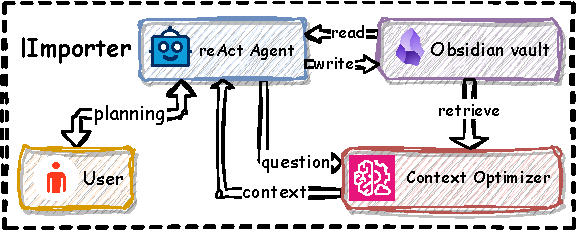
\includegraphics[width=0.85\textwidth]{figures/limporter.pdf}
    \caption{Esquema general del flujo de trabajo del agente lImporter.}
    \label{fig:importer_schema}
\end{figure}

\section{Descripción del entorno}
El entorno de trabajo para este proyecto es Obsidian. A diferencia de otras herramientas basadas en la nube, el modelo de datos de Obsidian es simple y robusto: una carpeta local en el sistema de archivos del usuario que contiene todos los datos. Las notas se almacenan como archivos de texto plano en formato Markdown (`.md`), y pueden organizarse en una jerarquía de carpetas tradicional. Este enfoque garantiza la portabilidad, la longevidad y el control total del usuario sobre su información.

Una de las características más distintivas de Obsidian es su capacidad para visualizar las conexiones entre notas como un grafo de conocimiento. Cada nota es un nodo en el grafo, y los vínculos entre notas se representan como aristas. Esto permite al usuario descubrir relaciones emergentes y navegar por su conocimiento de una manera no lineal.

\begin{figure}[h]
    \centering
    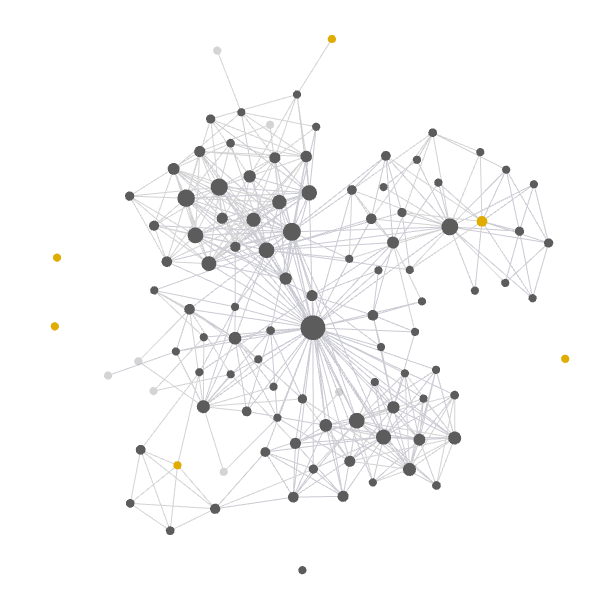
\includegraphics[width=0.8\textwidth]{figures/obsidian_kg_example.png}
    \caption{Ejemplo de la vista de grafo en Obsidian, mostrando nodos y sus interconexiones.}
    \label{fig:obsidian_graph}
\end{figure}

La creación de vínculos es fundamental para construir el grafo. En Obsidian, esto se logra mediante la sintaxis de \textit{wikilinks}, simplemente encerrando el nombre de otra nota entre dobles corchetes, por ejemplo, `[[Nota Destino]]`. Además de los vínculos simples, Obsidian soporta el concepto de \textbf{transclusión}, que permite incrustar el contenido de una nota (o una sección de ella) dentro de otra usando la sintaxis `![[Nota a Incrustar]]`. La transclusión crea un vínculo compuesto y fuerte, ya que el contenido de una nota se convierte en parte integral de otra, fomentando la atomicidad y la reutilización de la información.

\section{Detalles de Implementación}
Para la implementación de \textit{lImporter}, se propone un agente autónomo basado en el paradigma ReAct (Reasoning and Acting). Este agente está dotado de un conjunto de herramientas especializadas que le permiten interactuar directamente con la bóveda de Obsidian, leyendo su estructura, obteniendo el contenido de las notas y escribiendo nueva información.

La explicación de la arquitectura se realizará de manera \textit{top-down}. Se comenzará describiendo el funcionamiento general del agente, para luego profundizar en cada uno de sus componentes clave: el mecanismo de interacción con la bóveda y las estrategias para la obtención de contexto relevante.

\subsection{Agente reAct}
En el núcleo del sistema se encuentra un agente basado en el framework ReAct \parencite{yaoReActSynergizingReasoning2023}. Este paradigma permite a los modelos de lenguaje combinar el razonamiento (thought) con la acción (action). El agente opera en un ciclo donde, a partir de una tarea y una observación del entorno, razona sobre el siguiente paso a seguir, elige una herramienta de su repertorio, la ejecuta, y observa el resultado para informar su siguiente ciclo de razonamiento.

Siguiendo las mejores prácticas observadas en agentes avanzados como los utilizados para investigación o codificación (e.g. \textit{Deep Research}), se ha adoptado la estrategia \textit{Plan-and-Solve} \parencite{wangPlanandSolvePromptingImproving2023}. En lugar de actuar de forma impulsiva, el agente primero genera un plan detallado y paso a paso para resolver la tarea. El usuario tiene la opción de revisar, confirmar y dar retroalimentación sobre el plan generado antes de su ejecución. Este enfoque de \textit{human-in-the-loop} combina la eficiencia del planeamiento autónomo con la supervisión y el direccionamiento estratégico del usuario.

Para la implementación del agente se utiliza la familia de modelos Gemini de Google, debido a su alta capacidad, accesibilidad y, de manera crucial, su soporte nativo para \textit{function calling}, un mecanismo que se detallará a continuación.

\subsection{Interacción con la bóveda}
La capacidad del agente para leer y escribir archivos en la bóveda es posible gracias al uso de la API de Obsidian, orquestada a través de \textit{Function Calling}. Esta técnica puede ser entendida como un caso particular de \textit{style prompting} que emplea decodificación restringida (\textit{constrained decoding}) para forzar al modelo de lenguaje a generar una salida que se adhiere estrictamente a una gramática o formato predefinido \parencite{gengGrammarConstrainedDecodingStructured2024}.

En el caso de la API de Gemini, esta restricción obliga al modelo a producir una salida en formato JSON que se corresponde con la firma de una de las funciones (herramientas) disponibles. Se aprovecha esta capacidad para mejorar la fiabilidad del agente. Por ejemplo, al definir los parámetros de una función, se puede utilizar el tipo de dato `ENUM` para restringir las entradas a un conjunto de valores válidos (e.g., una lista de carpetas o archivos existentes), evitando así que el modelo intente operar sobre rutas inválidas o alucinadas.

\subsubsection{Lectura}
Para la lectura de información de la bóveda, el agente dispone de dos herramientas principales:
\begin{itemize}
    \item \texttt{tree(path)}: Esta función recibe la ruta a una carpeta raíz y devuelve una representación textual de la estructura de directorios y archivos contenida en ella, de forma análoga al comando \texttt{tree} de la línea de comandos. Esto permite al agente obtener una visión global de la organización de la bóveda.
    \item \texttt{read(path)}: Esta función recibe la ruta a un archivo Markdown (`.md`) existente y devuelve su contenido completo como texto.
\end{itemize}
 
\subsubsection{Escritura}
Un desafío común en los agentes que interactúan con sistemas de archivos es la tendencia del modelo a generar rutas de archivo incorrectas o con nombres similares pero no idénticos a los existentes. Para mitigar este problema, la capacidad de escritura se ha separado en dos funciones distintas:
\begin{itemize}
    \item \texttt{mkdir(path)}: Permite al agente crear un nuevo directorio en una ubicación específica de la bóveda, asegurando que la estructura de carpetas deseada exista antes de intentar escribir un archivo.
    \item \texttt{write(path, content)}: Crea un nuevo archivo o sobrescribe el contenido de uno existente. El parámetro \texttt{path} de esta función se beneficia directamente de la decodificación restringida, ya que se puede guiar al modelo para que elija entre rutas sugeridas o siga un formato válido, reduciendo drásticamente los errores.
\end{itemize}
 
\subsubsection{Obtencion de contexto}
Para que el agente pueda tomar decisiones informadas, como determinar dónde crear una nueva nota o con qué notas existentes vincularla, necesita un contexto relevante de la bóveda. Dado que el contenido total de la bóveda puede exceder fácilmente la ventana de contexto del modelo, se utiliza un enfoque de divide y vencerás.

Se propone una función que recibe un conjunto de archivos y un límite de tokens. Si el contenido combinado de los archivos excede el límite, el conjunto se divide recursivamente por la mitad hasta que los fragmentos resultantes son lo suficientemente pequeños. Una vez que un fragmento cabe en la ventana de contexto, un modelo de lenguaje se encarga de extraer la información relevante de él. La naturaleza de esta información relevante se define por un nivel de \textbf{granularidad} especificado por el usuario (en \cite{chenDenseRetrievalWhat2024} se analiza la optimalidad de selección de diferentes casos de estos).

Esta idea está inspirada en la técnica propuesta en \cite{shenQwenLongCPRS$infty$LLMsDynamic2025}. De manera similar, se proponen tres niveles de granularidad:
\begin{itemize}
    \item \textbf{Paragraph}: Ideal para obtener resúmenes y el sentido general de un documento.
    \item \textbf{Sentence}: Extremadamente útil para identificar afirmaciones específicas y recuperar relaciones entre conceptos.
    \item \textbf{Keyword}: Perfecto para la extracción de entidades nombradas y conceptos clave.
\end{itemize}

A continuación se presenta un pseudocódigo del proceso de obtención de contexto:

\begin{verbatim}
function getContext(files, token_limit, granularity):
    if total_tokens(files) <= token_limit:
        return extract_info(files, granularity)
    else:
        mid = floor(len(files) / 2)
        part1 = files[0:mid]
        part2 = files[mid:len(files)]
        
        context1 = getContext(part1, token_limit, granularity)
        context2 = getContext(part2, token_limit, granularity)
        
        return combine(context1, context2)
\end{verbatim}

\subsection{Sobre la versatibilidad del sistema}
Un objetivo clave de \textit{lImporter} es su versatilidad para integrarse en diversos flujos de trabajo. El agente debe ser útil tanto para un usuario que desea construir una base de conocimiento densamente interconectada, generando múltiples relaciones y resúmenes, como para otro que simplemente quiere archivar un nuevo concepto de forma aislada, sin crear ningún vínculo.

La arquitectura basada en un agente ReAct y el sistema de obtención de contexto granular sustentan esta flexibilidad. El agente puede recibir instrucciones para ser exhaustivo en la búsqueda de conexiones o, por el contrario, para limitarse a crear una nota y guardarla en una carpeta específica. Sin embargo, esta versatilidad conlleva un incremento en la labor manual de configuración inicial, ya que el comportamiento del agente se define en gran medida a través de un archivo de instrucciones proporcionado por el usuario.

\chapter{Experimentos}\label{chapter:implementation}
En este capítulo se presentan una serie de experimentos diseñados para evaluar el rendimiento y las capacidades del agente \textit{lImporter}. Es importante aclarar que no se realizó un análisis holístico y cuantitativo del sistema. En su lugar, se optó por explorar distintos casos de uso que demuestran la versatilidad de la herramienta y ponen de manifiesto las interesantes posibilidades que surgen al integrar un agente de lenguaje autónomo en una bóveda de conocimiento de Obsidian.

\section{Base estructurada sobre Harry Potter}
En el primer experimento, se utilizó la versatilidad del agente para una tarea clásica: la creación de una base de conocimientos estructurada sobre el universo de Harry Potter. El objetivo era proporcionar al agente los textos de los libros y pedirle que generara notas para personajes, lugares y conceptos clave, vinculándolos entre sí. Este caso de uso potencia a Obsidian como una herramienta para la exploración visual del conocimiento a través de su vista de grafo.

Es relevante mencionar que, por defecto, Obsidian no muestra etiquetas en las aristas del grafo, lo que dificulta la interpretación de la naturaleza de las relaciones. Para solventar esto, se utilizó un plugin de la comunidad que añade dicha funcionalidad. El grafo resultante, como se muestra en la Figura \ref{fig:hp_graph}, fue creado exitosamente. Una prueba de la correcta identificación de la relevancia de los conceptos se observa en el tamaño de los nodos: los nodos correspondientes a \textit{Harry Potter} y \textit{Hogwarts} son visiblemente más grandes, indicando un mayor número de conexiones y, por tanto, una mayor centralidad en la narrativa.

\begin{figure}[h]
    \centering
    % \includegraphics[width=0.8\textwidth]{path/to/hp_graph.png}
    \fbox{\parbox[c][15em][c]{0.8\textwidth}{\centering \huge Placeholder: \\ Grafo de conocimiento de Harry Potter generado por el agente}}
    \caption{Grafo resultante del experimento de Harry Potter, mostrando la centralidad de nodos clave.}
    \label{fig:hp_graph}
\end{figure}

% \subsection{Consideraciones}
% Placeholder para el análisis del experimento.
% - Analizar la calidad de las notas generadas.
% - Evaluar la precisión de los vínculos creados.
% - Discutir los desafíos encontrados, como la desambiguación de entidades.
% \textit{Placeholder para el análisis detallado del experimento.}

\section{Añadiendo articulos a una \textit{Wiki} tecnológica}
Este experimento se diseñó para simular el mantenimiento y crecimiento de una base de conocimiento existente. Se partió de una bóveda de Obsidian que funcionaba como una \textit{wiki} personal sobre temas de tecnología (programación, inteligencia artificial, etc.). Progresivamente, se le proporcionaron al agente nuevos artículos, acompañados de un breve resumen en audio describiendo su contenido.

El objetivo era doble. Por un lado, se buscaba demostrar que el agente es capaz de analizar el nuevo contenido, comprenderlo en el contexto de la bóveda existente y determinar correctamente con qué notas preexistentes debía vincularlo (Figura \ref{fig:wiki_cluster}). Por otro lado, y de igual importancia, se quería verificar que el agente no siempre establece conexiones. Si un nuevo artículo trata sobre un tema completamente ajeno a lo que ya existe en la bóveda, el resultado deseable es que se cree una nota aislada, sin vínculos forzados o incorrectos (Figura \ref{fig:wiki_isolated}). Este comportamiento es crucial para mantener la integridad y la calidad del grafo de conocimiento.

\begin{figure}[h]
    \centering
    % \includegraphics[width=0.45\textwidth]{path/to/wiki_cluster.png}
    \fbox{\parbox[c][15em][c]{0.45\textwidth}{\centering \huge Placeholder: \\ Cluster de notas relacionadas}}
    \caption{Nuevas notas integradas y conectadas con el conocimiento existente en la wiki.}
    \label{fig:wiki_cluster}
\end{figure}
\begin{figure}[h]
    \centering
    % \includegraphics[width=0.45\textwidth]{path/to/wiki_isolated.png}
    \fbox{\parbox[c][15em][c]{0.45\textwidth}{\centering \huge Placeholder: \\ Notas aisladas sin conexión}}
    \caption{Nuevas notas añadidas que permanecen como \textit{islas} de conocimiento, al no tener relación directa con el contenido previo.}
    \label{fig:wiki_isolated}
\end{figure}

% \subsection{Consideraciones}
% Placeholder para el análisis del experimento.
% - Analizar la tasa de acierto en la vinculación.
% - Evaluar los casos en los que decidió no vincular.
% - Discutir cómo la granularidad del contexto influyó en la decisión.
% \textit{Placeholder para el análisis detallado del experimento.}

\section{Projects, Areas, Resources, Archived}
Este experimento refleja un caso de uso más cotidiano y de productividad personal, siguiendo la metodología P.A.R.A. (Projects, Areas, Resources, Archived) popularizada por Tiago Forte en su libro \textit{Building a Second Brain} \cite{forteBuildingSecondBrain2022}. El objetivo era evaluar si el sistema puede ser utilizado para mantener una bóveda organizada bajo esta estructura, siguiendo instrucciones de voz.

Se probó la capacidad del agente para realizar tareas como:
\begin{itemize}
    \item Incluir nuevos archivos (recursos) en la bóveda, clasificándolos correctamente en la carpeta `Resources`.
    \item Vincular estos nuevos recursos con notas existentes en las carpetas `Projects` o `Areas`.
    \item Sintetizar información a partir de varias notas existentes para generar un nuevo resumen o una nota de trabajo.
\end{itemize}
Este escenario pone a prueba no solo la interacción con el sistema de archivos, sino también la capacidad del agente para comprender la intención del usuario y ejecutar flujos de trabajo más complejos y estructurados.

% \subsection{Consideraciones}
% Placeholder para el análisis del experimento.
% - Evaluar la capacidad del agente para seguir instrucciones complejas y multi-paso.
% - Analizar la correcta clasificación de notas en la estructura P.A.R.A.
% - Discutir la calidad de la información sintetizada.
% \textit{Placeholder para el análisis detallado del experimento.}

\section{Note augmented \textit{LLMs} are computationally universal}
Este último experimento, de naturaleza más teórica, se inspira en la idea de que los modelos de lenguaje, cuando se aumentan con una memoria externa, pueden volverse computacionalmente universales \parencite{schuurmansMemoryAugmentedLarge2023}.

Para explorar esta idea, se le pidió al agente que evaluara la Conjetura de Collatz para un número dado, utilizando una nota de Obsidian como su \textit{memoria de trabajo} o registro. En cada paso de la secuencia, el agente leía el número actual de la nota, calculaba el siguiente número, y sobrescribía la nota con el nuevo valor.

Se evaluó el caso para $n=10$, que se resolvió correctamente en 6 iteraciones (Figuras \ref{fig:collatz_code} y \ref{fig:collatz_diff}). También se evaluaron casos más largos como $n=11$ (14 iteraciones) y $n=27$ (111 iteraciones). Este último caso excedió los límites de cuota de la API y requirió reiniciar el proceso, lo cual demostró una capacidad emergente del sistema: la posibilidad de dejar una tarea y seguirla luego, ya que el estado se preserva en la nota de Obsidian.

La intuición subyacente es que la capacidad de releer el estado desde un archivo fiable reduce drásticamente la probabilidad de error en un proceso iterativo largo, de manera análoga a cómo una CPU depende de leer y escribir correctamente en sus registros. En este caso se usó un modelo potente en razonamiento algebraico (Gemini 2.5 Flash). Si bien un modelo más modesto podría fallar en esta tarea matemática, la misma arquitectura podría permitirle automatizar con alta fiabilidad otra tarea iterativa que se alinee con sus fortalezas (por ejemplo, un análisis de sentimiento refinado a lo largo de múltiples revisiones), siempre que sea proficiente en las operaciones básicas de leer y escribir en su memoria externa.

\begin{figure}[h]
    \centering
    % \includegraphics[width=0.45\textwidth]{path/to/collatz_code.png}
    \fbox{\parbox[c][15em][c]{0.45\textwidth}{\centering \huge Placeholder: \\ Contenido de la nota de Collatz}}
    \caption{Estado de la nota de trabajo durante la evaluación de Collatz.}
    \label{fig:collatz_code}
\end{figure}
\begin{figure}[h]
    \centering
    % \includegraphics[width=0.45\textwidth]{path/to/collatz_diff.png}
    \fbox{\parbox[c][15em][c]{0.45\textwidth}{\centering \huge Placeholder: \\ Diff entre iteraciones}}
    \caption{Diferencia en el contenido de la nota entre dos pasos de la iteración.}
    \label{fig:collatz_diff}
\end{figure}

% \subsection{Consideraciones}
% Placeholder para el análisis del experimento.
% - Discutir la fiabilidad del proceso iterativo.
% - Analizar los fallos y cómo la relectura del estado ayuda a corregirlos.
% - Reflexionar sobre las implicaciones de usar una bóveda como memoria externa para tareas computacionales complejas.
% \textit{Placeholder para el análisis detallado del experimento.}